\documentclass{wfiisul}

\usepackage[utf8]{inputenc}
\usepackage{amsmath}
\usepackage{tabularx}
\usepackage[hidelinks]{hyperref}
\usepackage{afterpage}

%\usepackage{pdflscape}
%\usepackage{afterpage}
%\usepackage{changepage}
%\usepackage{caption}
%\usepackage{rotating} %for sidewisetable
%\usepackage{makecell}
%\usepackage{boldline}
%\usepackage{amsthm}
%\usepackage{amsopn}
%\usepackage{wrapfig}
%\usepackage[table]{xcolor}

\usepackage{framed}
\usepackage{listings}
\usepackage[most]{tcolorbox}
\usepackage{hyphenat}

\hyphenation{pra-cy}

\begin{document}

\tytul{Zastosowanie ABM do analizy procesu formowania opinii w wielowymiarowej przestrzeni opinii}

\autor{Mateusz Borowiec}
\nralbumu{382765}

\promotor{Dr hab. Tomasz Gwizdałła, prof. UŁ}
\katedra{Systemów Inteligentnych}

\kierunek{informatyka}

\specjalnosc{informatyka stosowana}
\typpracy{magisterska}
\sciezka{Sztuczna inteligencja}

\stronatytulowa

%%%%%%%%%%%%%%%%%%%%%%%%%%%%%%%%%%%%%%%%%%%%%%%%%%%%%%%%%%%%%%%%%%%%%%%%%%%%%%%%%%%%%%%%%%%%%%%%%%%%%%%%%%%%%%%%%%%%%%%%%%%%%%%%%%%%%%%%%%%%%%%%%%%%%%%%%%%%%%%%%%%%%%%%%%%%%%%%%%%%%%%%%%%%%%%%%%%%%%%%%%%%%%%%%%


\chapter{Wstęp}



%%%%%%%%%%%%%%%%%%%%%%%%%%%%%%%%%%%%%%%%%%%%%%%%%%%%%%%%%%%%%%%%%%%%%%%%%%%%%%%%%%%%%%%%%%%%%%%%%%%%%%%%%%%%%%%%%%%%%%%%%%%%%%%%%%%%%%%%%%%%%%%%%%%%%%%%%%%%%%%%%%%%%%%%%%%%%%%%%%%%%%%%%%%%%%%%%%%%%%%%%%%%%%%%%%

\chapter{Podstawy teoretyczne}

TYMCZASOWY TEKST Z OPISU PRACY

Metody agentowe (Agent Based Modelling) są jedną z popularnych metod analizy wielu procesów zachodzących w społecznościach. 
Jednym z takich procesów jest rozprzestrzenianie się opinii, przy czym opinia może być reprezentowana w różny sposób. 
W prezentowanej pracy ma ona być przedstawiona w formie położenia w znormalizowanej przestrzeni wielowymiarowej (przykładem takiej przestrzeni jest dwuwymiarowy diagram Nolana). 
Społeczność zostanie przedstawiona w formie typowych grafów społecznościowych (Barabasi-Albert, Watts-Strogatz, Erdos-Renyi). 
Celem pracy jest określenie stanów końcowych takich modeli dla wybranych funkcji modyfikacji opinii oraz czasów dojścia do tych stanów. 
Wśród pytań, które pojawiają się w trakcie rozwiązywania takiego problemu, są takie jak: 
pytanie o istnienie (dla danej funkcji modyfikacji) krytycznej wielkości próbki, dla której struktura rozwiązania ulega zmianie (np. pojawiają się odstępstwa od jednomyślności) 
czy pytanie o możliwość włączenia czynników zewnętrznych.

%%%%%%%%%%%%%%%%%%%%%%%%%%%%%%%%%%%%%%%%%%%%%%%%%%%%%%%%%%%%%%%%%%%%%%%%%%%%%%%%%%%%%%%%%%%%%%%%%%%%%%%%%%%%%%%%%%%%%%%%%%%%%%%%%%%%%%%%%%%%%%%%%%%%%%%%%%%%%%%%%%%%%%%%%%%%%%%%%%%%%%%%%%%%%%%%%%%%%%%%%%%%%%%%%%

\chapter{Opis metod (algorytmy, założenia, warunki graniczne)}

Agent posiada następujące parametry:

\begin{table}[htbp]
  \centering
  \begin{tabular}{c|c|c}
    \hline
    Zmienna & Zakres wartości & Rozkład \\
    \hline
    Wpływ na innych & 0-1 & równomierny \\
    Elastyczność jednostki & 0,1-1 & beta \\
    Opinia początkowa & 0-1 & równomierny \\
  \end{tabular}
  \caption{Parametry agenta}
  \label{tab:agent_parameters}
\end{table}

Aktualizacja opinii składa się z następujących zmiennych:

\begin{table}[htbp]
  \centering
  \begin{tabular}{c|c}
    \hline
    Zmienna & Zakres wartości \\
    \hline
    Średnia opinii sąsiadów & 0-1 \\
    Srednia wpływu sąsiadów & 0-1 \\
    Udział znajomych agenta w populacji & 0-1 \\
    Odległość opinii agenta i średniej znajomych & 0-1 \\
    Modyfikator środka rozkładu & Elastyczność agenta\\% * (udział znajomych agenta w populacji + wpływ sąsiadów) = [0-1] * ([0-1] + [0-1]) \\
  \end{tabular}
  \caption{Parametry aktualizacji opinii}
  \label{tab:opinion_update_parameters}
\end{table}

\section{Rozkład trójkątny}

Opinia sąsiadów:
\begin{itemize}
  \item średnia opinii sąsiadów: 0-1
  \item średnia wpływu sąsiadów: 0-1
\end{itemize}

Centrum rozkładu trójkątnego: (stopień jednostki + średnia wpływu sąsiadów) * elastyczność jednostki

Minimum rozkładu: opinia jednostki

Maksimum rozkładu: średnia opinii sąsiadów

Odległość między opiniami = abs (opinia jednostki — średnia opinii sąsiadów)

\section{Nowy modyfikator środka rozkładu}

Elastyczność agenta * średnia ([udział znajomości agenta w populacji, wpływ sąsiadów]) = [0-1] * ([0-1] * [0-1] / 2) = [0-1] * [0-1] = [0-1].

Średnia wpływu sąsiadów będzie średnią ważoną.

%%%%%%%%%%%%%%%%%%%%%%%%%%%%%%%%%%%%%%%%%%%%%%%%%%%%%%%%%%%%%%%%%%%%%%%%%%%%%%%%%%%%%%%%%%%%%%%%%%%%%%%%%%%%%%%%%%%%%%%%%%%%%%%%%%%%%%%%%%%%%%%%%%%%%%%%%%%%%%%%%%%%%%%%%%%%%%%%%%%%%%%%%%%%%%%%%%%%%%%%%%%%%%%%%%

\chapter{Opis technologii wykorzystanych w pracy}

W pracy został wykorzystany język Python do implementacji zarówno sieci społecznych, zapisu wyników, jak i wykresów obrazujących wyniki. 
Główną biblioteką wykorzystywaną do implementacji sieci społecznych jest biblioteka NetworkX. 
Biblioteką do tworzenia wykresów została biblioteka Matplotlib. 
Do odczytu / zapisu plików CSV została użyta biblioteka `csv`. 

%%%%%%%%%%%%%%%%%%%%%%%%%%%%%%%%%%%%%%%%%%%%%%%%%%%%%%%%%%%%%%%%%%%%%%%%%%%%%%%%%%%%%%%%%%%%%%%%%%%%%%%%%%%%%%%%%%%%%%%%%%%%%%%%%%%%%%%%%%%%%%%%%%%%%%%%%%%%%%%%%%%%%%%%%%%%%%%%%%%%%%%%%%%%%%%%%%%%%%%%%%%%%%%%%%

\chapter{Opis implementacji}

\section{Klasa Network}

Każda sieć społeczna składa się z grafu NetworkX oraz listy agentów, przypisanych do każdego wierzchołka. 
Typ aktualizacji opinii jest również zdefiniowany w klasie. 
Ponadto, do celów logowania, klasa zawiera nazwę sieci społecznej. 

\section{Klasa Agent}

Każdy agent ma następujące parametry:
\begin{itemize}
  \item Wpływ na innych (influence) - Ten parametr osiąga wartości 0-1 i określa wartość wpływu na innych agentów
  \item Elastyczność (flexibility) - Osiąga wartości 0-1 i określa podatność agenta na zmianę opinii pod wpływem swoich sąsiadów
  \item Opinia (opinion) - Osiąga wartości 0-1 i określa wartość opinii agenta w zależności od opinii sąsiadów
\end{itemize}

%%%%%%%%%%%%%%%%%%%%%%%%%%%%%%%%%%%%%%%%%%%%%%%%%%%%%%%%%%%%%%%%%%%%%%%%%%%%%%%%%%%%%%%%%%%%%%%%%%%%%%%%%%%%%%%%%%%%%%%%%%%%%%%%%%%%%%%%%%%%%%%%%%%%%%%%%%%%%%%%%%%%%%%%%%%%%%%%%%%%%%%%%%%%%%%%%%%%%%%%%%%%%%%%%%

\chapter{Opis wykonanych w ramach pracy badań, symulacji, eksperymentów}


\section{Model początkowy}

Początkowo zostały zaimplementowane trzy sieci: Barabasi-Albert, Erdos-Renyi, Watts-Strogatz. 
Ich opinie zmieniały się w zależności od opinii sąsiadów. 
Aktualizacja współrzędnych modelu była zmieniana w jednej iteracji równocześnie dla wszystkich węzłów, co doprowadziło do szybkiego zbiegania agentów do centrum. 

\section{Pierwsze poprawki}

Po pierwszych próbach wprowadzone zostały zmiany. Każdy agent musi mieć dar przekonywania, który pozwoli mu wpływać na innych agentów. 
% 1a. Huby mają większy dar przekonywania
Ponadto huby powinny mieć większy dar przekonywania. Aby uzyskać taki efekt, należy zwiększyć siłę oddziaływania węzłów z dużą liczbą sąsiadów. 
% 1b. Dar przekonywania nie zależy od rangi (stopnia) wierzchołka
Dar przekonywania nie powinien zależeć od stopnia wierzchołka, ponieważ nie są to wielkości skorelowane. 
% 1c. Konserwatyzm osobnika
Ponadto, każdy agent powinien mieć właściwość zwaną elastycznością, która zwiększa prawdopodobieństwo, że dany agent zmieni swoją opinię. 
% 2. Wyliczyliśmy średnią pozycję sąsiadów:
% 2a Gdzie i z jakim prawdopodobieństwem może przesunąć się osobnik?
% 2b. Jak zapisać zmianę energii związaną z potencjalną zmianą miejsca w przestrzeni rozwiązań?
% 2c. Z małym prawdopodobieństwem (wsp. konserwatyzmu) osobnik godzi się zmienić swoją opinię
% 2d. Załóżmy, że istnieje parametr \beta na poziomie 0.1, takie, że zmianę pozycji osobnika losujemy na prostej od jego aktualnej pozycji do położenia średniego.
%     Losujemy z rozkładu wykładniczego o średniej \beta*odległość(obiekt, średnia sąsiadów)
Zaszła również potrzeba zmiany wzoru aktualizacji opinii, ponieważ poprzednia powodowała zbyt szybkie zbieganie opinii do jednego centrum. 

\subsection{Zmieniona implementacja}

Na nowo zaimplementowany agent ma trzy własności — opinię, elastyczność zmiany opinii i wpływ na innych. 
Opinia agenta na początku jest losowana z rozkładu równomiernego, podobnie jak wpływ na innych. 
Elastyczność z kolei jest losowana z rozkładu beta tak, żeby była względnie mała. 
Opinie są aktualizowane, bazując na rozkładzie trójkątnym oraz własnościach agenta i jego sąsiadów. 
Wyliczana jest średnia opinia sąsiadów oraz średnia ich wpływu. 
Następnie obliczany jest udział sąsiadów agenta w ogólnej liczbie węzłów, który bierze udział w przesuwaniu środka rozkładu. 
Przesunięcie obliczane jest wg wzoru: 
przesunięcie = elastyczność agenta * (udział sąsiadów agenta w populacji + wpływ sąsiadów) 

Sumowanie wpływu sąsiadów z udziałem sąsiadów agenta w populacji powoduje, że na agenta z większą ilością sąsiadów wywierany jest większy wpływ. 
Z drugiej strony, na odizolowanych osobników wywierany jest mniejszy wpływ, co powoduje, że 'okopują' się oni w swoich poglądach. 
Z kolei elastyczność agenta we wzorze pozwala ograniczyć wpływ otoczenia na danego agenta. 
 
Rezultat jest taki, że huby mają duży wpływ na bliskie poglądowo węzły, zacieśniając je coraz bardziej, natomiast węzły z małą liczbą sąsiadów przesuwają się w kierunku huba dużo wolniej. 

\section{Rozwinięcie badań}

% Obraz położenia/gęstości punktów w funkcji numeru iteracji
% Czy zbieganie zależy od liczby osobników w populacji
Poprawa w działaniu symulacji prowadziła do dalszych badań. Należało zrobić obraz gęstości punktów w funkcji numeru iteracji i zbadać, czy zbieżność zależy od liczby osobników w populacji. 
% Niech metryką oceny populacji będzie numer iteracji, w której zarówno w jednym, jak i w drugim wymiarze punkty mieszczą się w przedziale o szerokości 0.1.
% Nazwijmy to stabilizacją.
Aby ocenić działanie symulacji, należało obliczyć numer iteracji, w której współrzędne punktów mieszczą się w przedziale o szerokości 0,1, co można uznać za stan stabilizacji. 
% Dla każdego rozmiaru populacji wykonajmy po 10 powtórzeń. Jaki jest czas stabilizacji dla rozmiaru populacji 20, 50, 100, 200, 500, 1000, ....
Dla każdego rozmiaru populacji zostały wykonane po 10 powtórzeń. Na tej podstawie obliczono średnią liczbę iteracji prowadzącą do stabilizacji symulacji dla danego rozmiaru populacji. 
Okazało się, że czas zbiegania symulacji rośnie logarytmicznie względem wielkości populacji, co pozwala przewidzieć czas zbiegania dla danego rozmiaru populacji. 

\section{Drugie poprawki}

Po wykonaniu badań na nowym modelu okazały się konieczne kolejne poprawki. 
% 1. Policzyc współrzędne neighbor_opinions nie jako średnią ale jako średnią ważoną z neighbor_influence
Należało policzyć współrzędne opinii sąsiadów jako średnią ważoną z wpływu sąsiadów. 
% 2. Testowo - policzyć to samo co do tej pory, ale ze zmienionym neighbor_opinions. Czy choć trochę się opóźni?
Należało sprawdzić, czy zmiana opinii sąsiadów opóźni zbieganie symulacji. 
% 3. I to jest kierunek - skoro trójkąt nic nie daje sprawdźmy rozkład wykładniczy. Jak? 
% 3a. Nowy punkt losowany jest na odcinku pomiędzy agent.opinion (ao) i neighbor_opinions (no), przy czym losujemy z rozkładu wykładniczego o średniej zależnej od influence i flexibility. 
%     Oczywiście, im silniejszy wpływ i oporność osobnika tym mniejszy ruch. 
Ponadto, należało zmienić rozkład losowania opinii osobnika, która miała być od teraz zależna od obecnej opinii osobnika i opinii sąsiadów, oraz elastyczności osobnika. 
% 3b. Jeśli ciągle punkty dla powiedzmy 50 agentów zbiegają się wprowadzamy współczynnik modyfikujący średnią rozkładu. Czyli mnożymy każdą średnią przez tę samą liczbę. 
%     Schodzimy w dół wg. schematu 0.5, 0.2 0.1, 0.05.
Jeżeli punkty w dalszym ciągu będzie zbiegać szybko, będzie trzeba wprowadzić współczynnik modyfikujący średnią rozkładu. 
% 3c. Patrzymy, czy w którymś wreszcie momencie agenci nie zaczną rozdzielać się na idących za dwoma "liderami". Jeśli tak, to mamy coś.
% 3d. Patrzymy na różnicę w zachowaniu dla różnych sieci i różnych wielkości (kiedy pojawia się dążenie do różnych punktów, ile jest tych punktów)
Należy zaobserwować różnicę w zachowaniu dla różnych sieci oraz zależnie od wielkości populacji. 
Będzie potrzeba przeanalizowania, czy agenci nie zaczną rozdzielać się na dwie lub więcej grup. 

\subsection{Wyniki dla zwykłej średniej i średniej ważonej}

Różnica między wynikami dla zwykłej średniej i średniej ważonej we wzorze aktualizacji opinii ukazują tabele poniżej. 

\subsubsection{Sieć Barabasi-Albert}

\begin{table}[htbp]
  \centering
  \begin{tabular}{c|c|c}
    \hline
    Populacja & Średnia zwykła & Średnia ważona \\
    \hline
    20 & 7.1 & 8.9 \\
    50 & 8.4 & 10.8 \\
    100 & 10.9 & 14.8 \\
    200 & 11.0 & 15.8 \\
    500 & 13.5 & 18.2 \\
    1000 & 13.4 & 19.8 \\
    2000 & 14.9 & 20.0 \\
    5000 & 15.2 & 20.0 \\
  \end{tabular}
  \caption{Barabasi-Albert}
  \label{tab:barabasi_albert}
\end{table}

\subsubsection{Sieć Watts-Strogatz}

\begin{table}[htbp]
  \centering
  \begin{tabular}{c|c|c}
    \hline
    Populacja & Średnia zwykła & Średnia ważona \\
    \hline
    20 & 8.6 & 9.1 \\
    50 & 10.8 & 12.3 \\
    100 & 13.3 & 16.9 \\
    200 & 14.9 & 19.2 \\
    500 & 16.6 & 20.0 \\
    1000 & 18.3 & 20.0 \\
    2000 & 19.5 & 20.0 \\
    5000 & 20.0 & 20.0 \\
  \end{tabular}
  \caption{Watts-Strogatz}
  \label{tab:watts_strogatz}
\end{table}

\subsubsection{Sieć Erdos-Renyi}

\begin{table}[htbp]
  \centering
  \begin{tabular}{c|c|c}
    \hline
    Populacja & Średnia zwykła & Średnia ważona \\
    \hline
    20 & 5.5 & 6.6 \\
    50 & 5.7 & 6.0 \\
    100 & 6.4 & 6.2 \\
    200 & 6.2 & 7.1 \\
    500 & 7.6 & 7.5 \\
    1000 & 7.6 & 8.5 \\
    2000 & 8.0 & 8.4 \\
    5000 & 8.5 & 9.6 \\
  \end{tabular}
  \caption{Erdos-Renyi}
  \label{tab:erdos_renyi}
\end{table}


\section{Współczynnik modyfikujący średnią rozkładu}

Dodatkowy współczynnik modyfikujący średnią rozkładu został dodany do funkcji aktualizującej opinię danego agenta. 
Okazało się, że współczynnik wynoszący 500 jest odpowiedni dla uzyskania więcej niż jednej zbieżnej grupy, przynajmniej dla sieci Wattsa-Strogatza i Barabasi-Alberta. 
W przypadku Erdos-Renyi nie powstaje więcej niż jedna grupa, prędzej pojawiają się "orbitujące" elementy populacji, znacznie oddalone od głównej grupy. 
Dla mniejszych współczynników populacja jest zbieżna do jednej grupy, a dla większych elementy przestają się grupować. 
Przykładowe rezultaty widoczne są poniżej. 

\begin{figure}
  \centering
  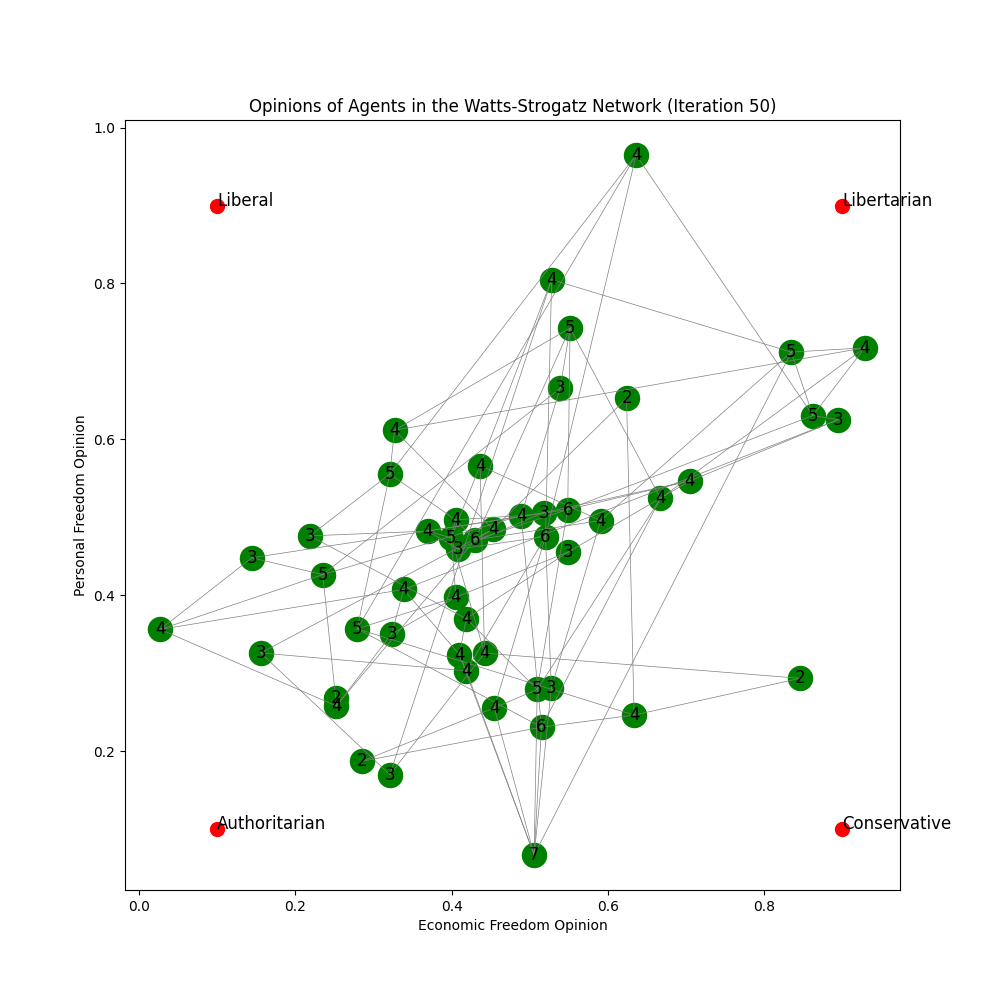
\includegraphics[width=0.5\textwidth]{img/Watts-Strogatz.png}
  \caption{Watts-Strogatz}
  \label{fig:Watts-Strogatz}
\end{figure}

\begin{figure}
  \centering
  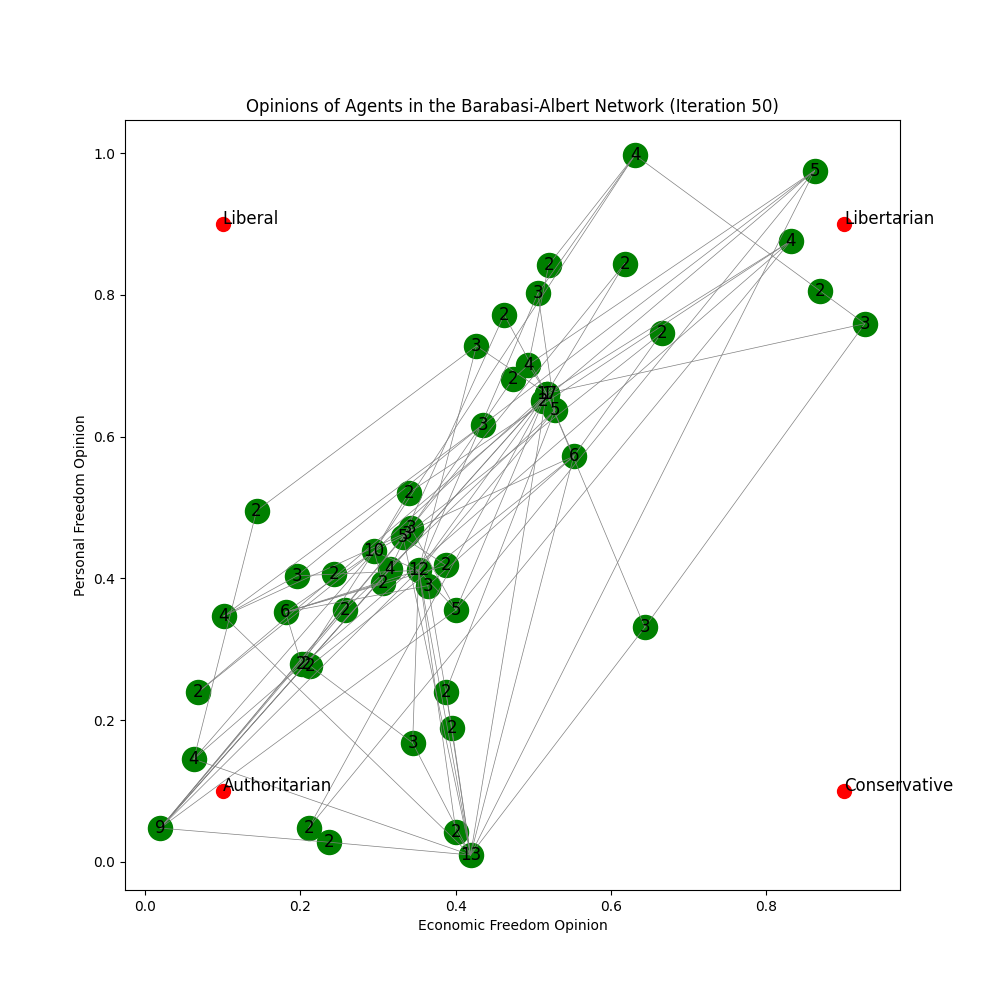
\includegraphics[width=0.5\textwidth]{img/Barabasi-Albert.png}
  \caption{Barabasi-Albert}
  \label{fig:Barabasi-Albert}
\end{figure}

\begin{figure}
  \centering
  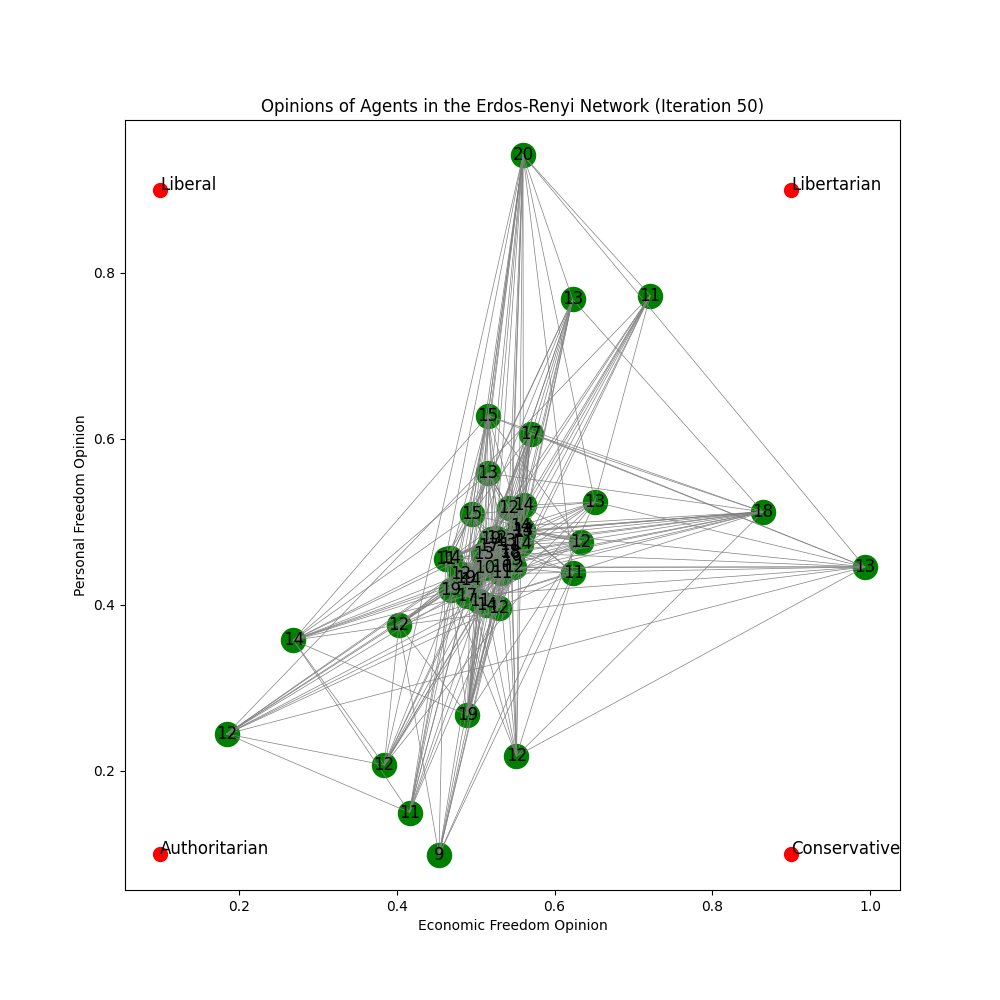
\includegraphics[width=0.5\textwidth]{img/Erdos-Renyi.png}
  \caption{Erdos-Renyi}
  \label{fig:Erdos-Renyi}
\end{figure}


\section{Analiza różnych współczynników modyfikujących średnią rozkładu}

Jako że współczynnik modyfikujący średnią rozkładu pozwolił na uzyskanie lepszych rezultatów niż do tej pory, przeprowadzono badania dla różnych wartości parametru, wyniki są w plikach CSV pod podanym linkiem. 

Przeprowadzone zostały obliczenia dla następujących wartości modyfikatora: [0,1, 0,2, 0,5, 1, 2, 5, 10, 20, 50, 100, 200, 500, 1000], 
oraz dla następujących wartości populacji: [20, 50, 100, 200, 500, 1000, 2000, 5000]. 

Niestety, niewiele z nich pozwoliło na uzyskanie więcej niż jednej grupy na wykresie. Wyniki widoczne poniżej. 

\begin{figure}
  \centering
  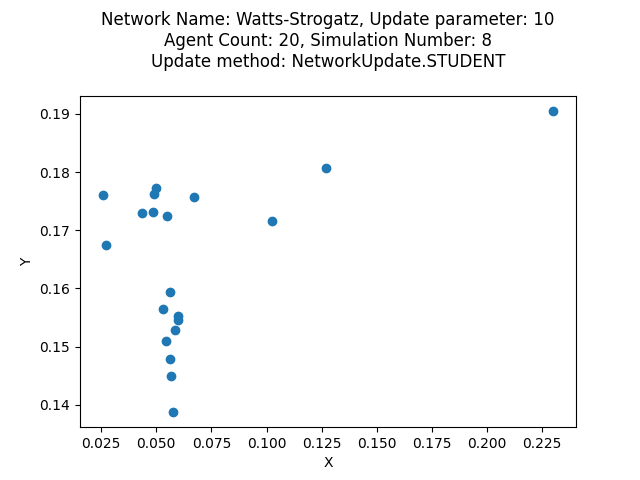
\includegraphics[width=0.5\textwidth]{img/watts_strogatz_10_20_8_student.png}
  \caption{watts strogatz 10 20 8 student}
  \label{fig:watts_strogatz_10_20_8_student}
\end{figure}

\begin{figure}
  \centering
  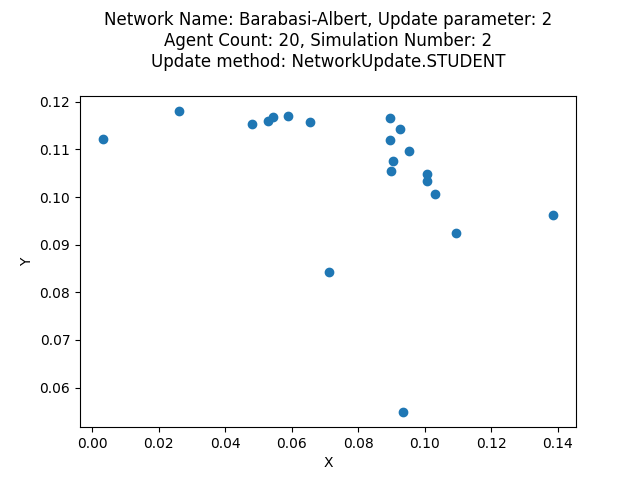
\includegraphics[width=0.5\textwidth]{img/barabasi_albert_2_20_2_student.png}
  \caption{barabasi albert 2 20 2 student}
  \label{fig:barabasi_albert_2_20_2_student}
\end{figure}

\begin{figure}
  \centering
  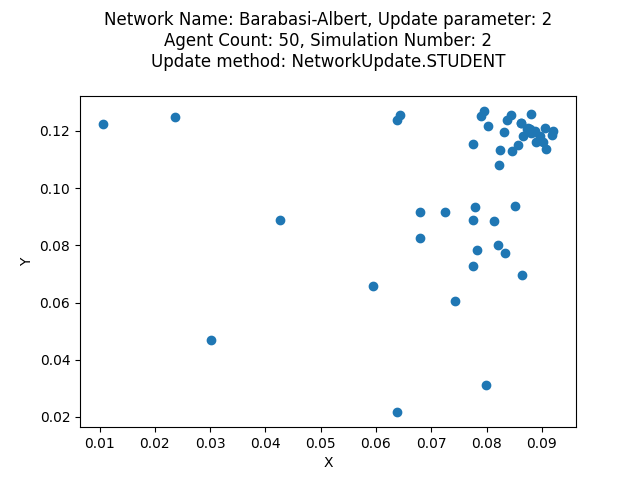
\includegraphics[width=0.5\textwidth]{img/barabasi_albert_2_50_2_student.png}
  \caption{barabasi albert 2 50 2 student}
  \label{fig:barabasi_albert_2_50_2_student}
\end{figure}

\begin{figure}
  \centering
  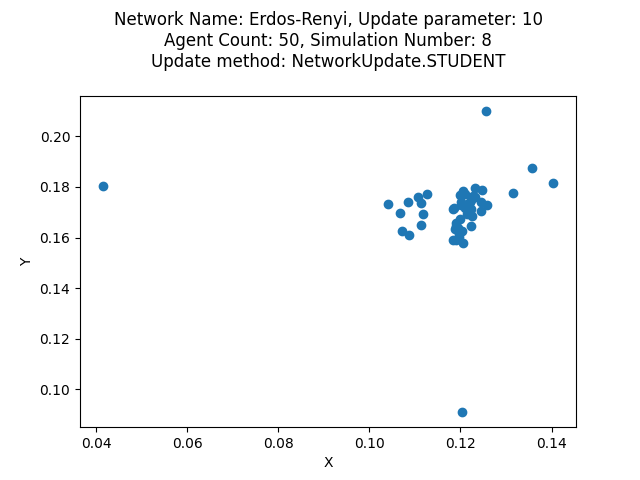
\includegraphics[width=0.5\textwidth]{img/erdos_renyi_10_50_8_student.png}
  \caption{erdos renyi 10 50 8 student}
  \label{fig:erdos_renyi_10_50_8_student}
\end{figure}

\begin{figure}
  \centering
  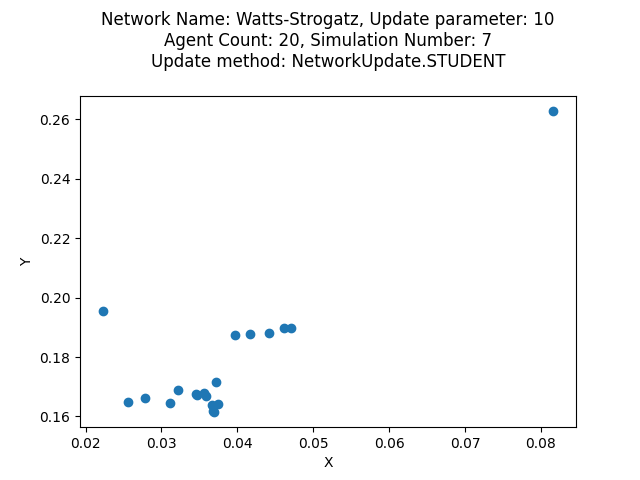
\includegraphics[width=0.5\textwidth]{img/watts_strogatz_10_20_7_student.png}
  \caption{watts strogatz 10 20 7 student}
  \label{fig:watts_strogatz_10_20_7_student}
\end{figure}

%%%%%%%%%%%%%%%%%%%%%%%%%%%%%%%%%%%%%%%%%%%%%%%%%%%%%%%%%%%%%%%%%%%%%%%%%%%%%%%%%%%%%%%%%%%%%%%%%%%%%%%%%%%%%%%%%%%%%%%%%%%%%%%%%%%%%%%%%%%%%%%%%%%%%%%%%%%%%%%%%%%%%%%%%%%%%%%%%%%%%%%%%%%%%%%%%%%%%%%%%%%%%%%%%%

\chapter{Analiza otrzymanych wyników}



%%%%%%%%%%%%%%%%%%%%%%%%%%%%%%%%%%%%%%%%%%%%%%%%%%%%%%%%%%%%%%%%%%%%%%%%%%%%%%%%%%%%%%%%%%%%%%%%%%%%%%%%%%%%%%%%%%%%%%%%%%%%%%%%%%%%%%%%%%%%%%%%%%%%%%%%%%%%%%%%%%%%%%%%%%%%%%%%%%%%%%%%%%%%%%%%%%%%%%%%%%%%%%%%%%

\chapter{Podsumowanie}

\listoftables
\listoffigures

\thebibliography{99}

\end{document}
